% Figure: the leaflet in 3D (PyVista renders; labels placed by the camera projection in leaflet3d_labels.tex).
\begin{tikzpicture}
\node[anchor=south west, inner sep=0] (a) at (0,0) {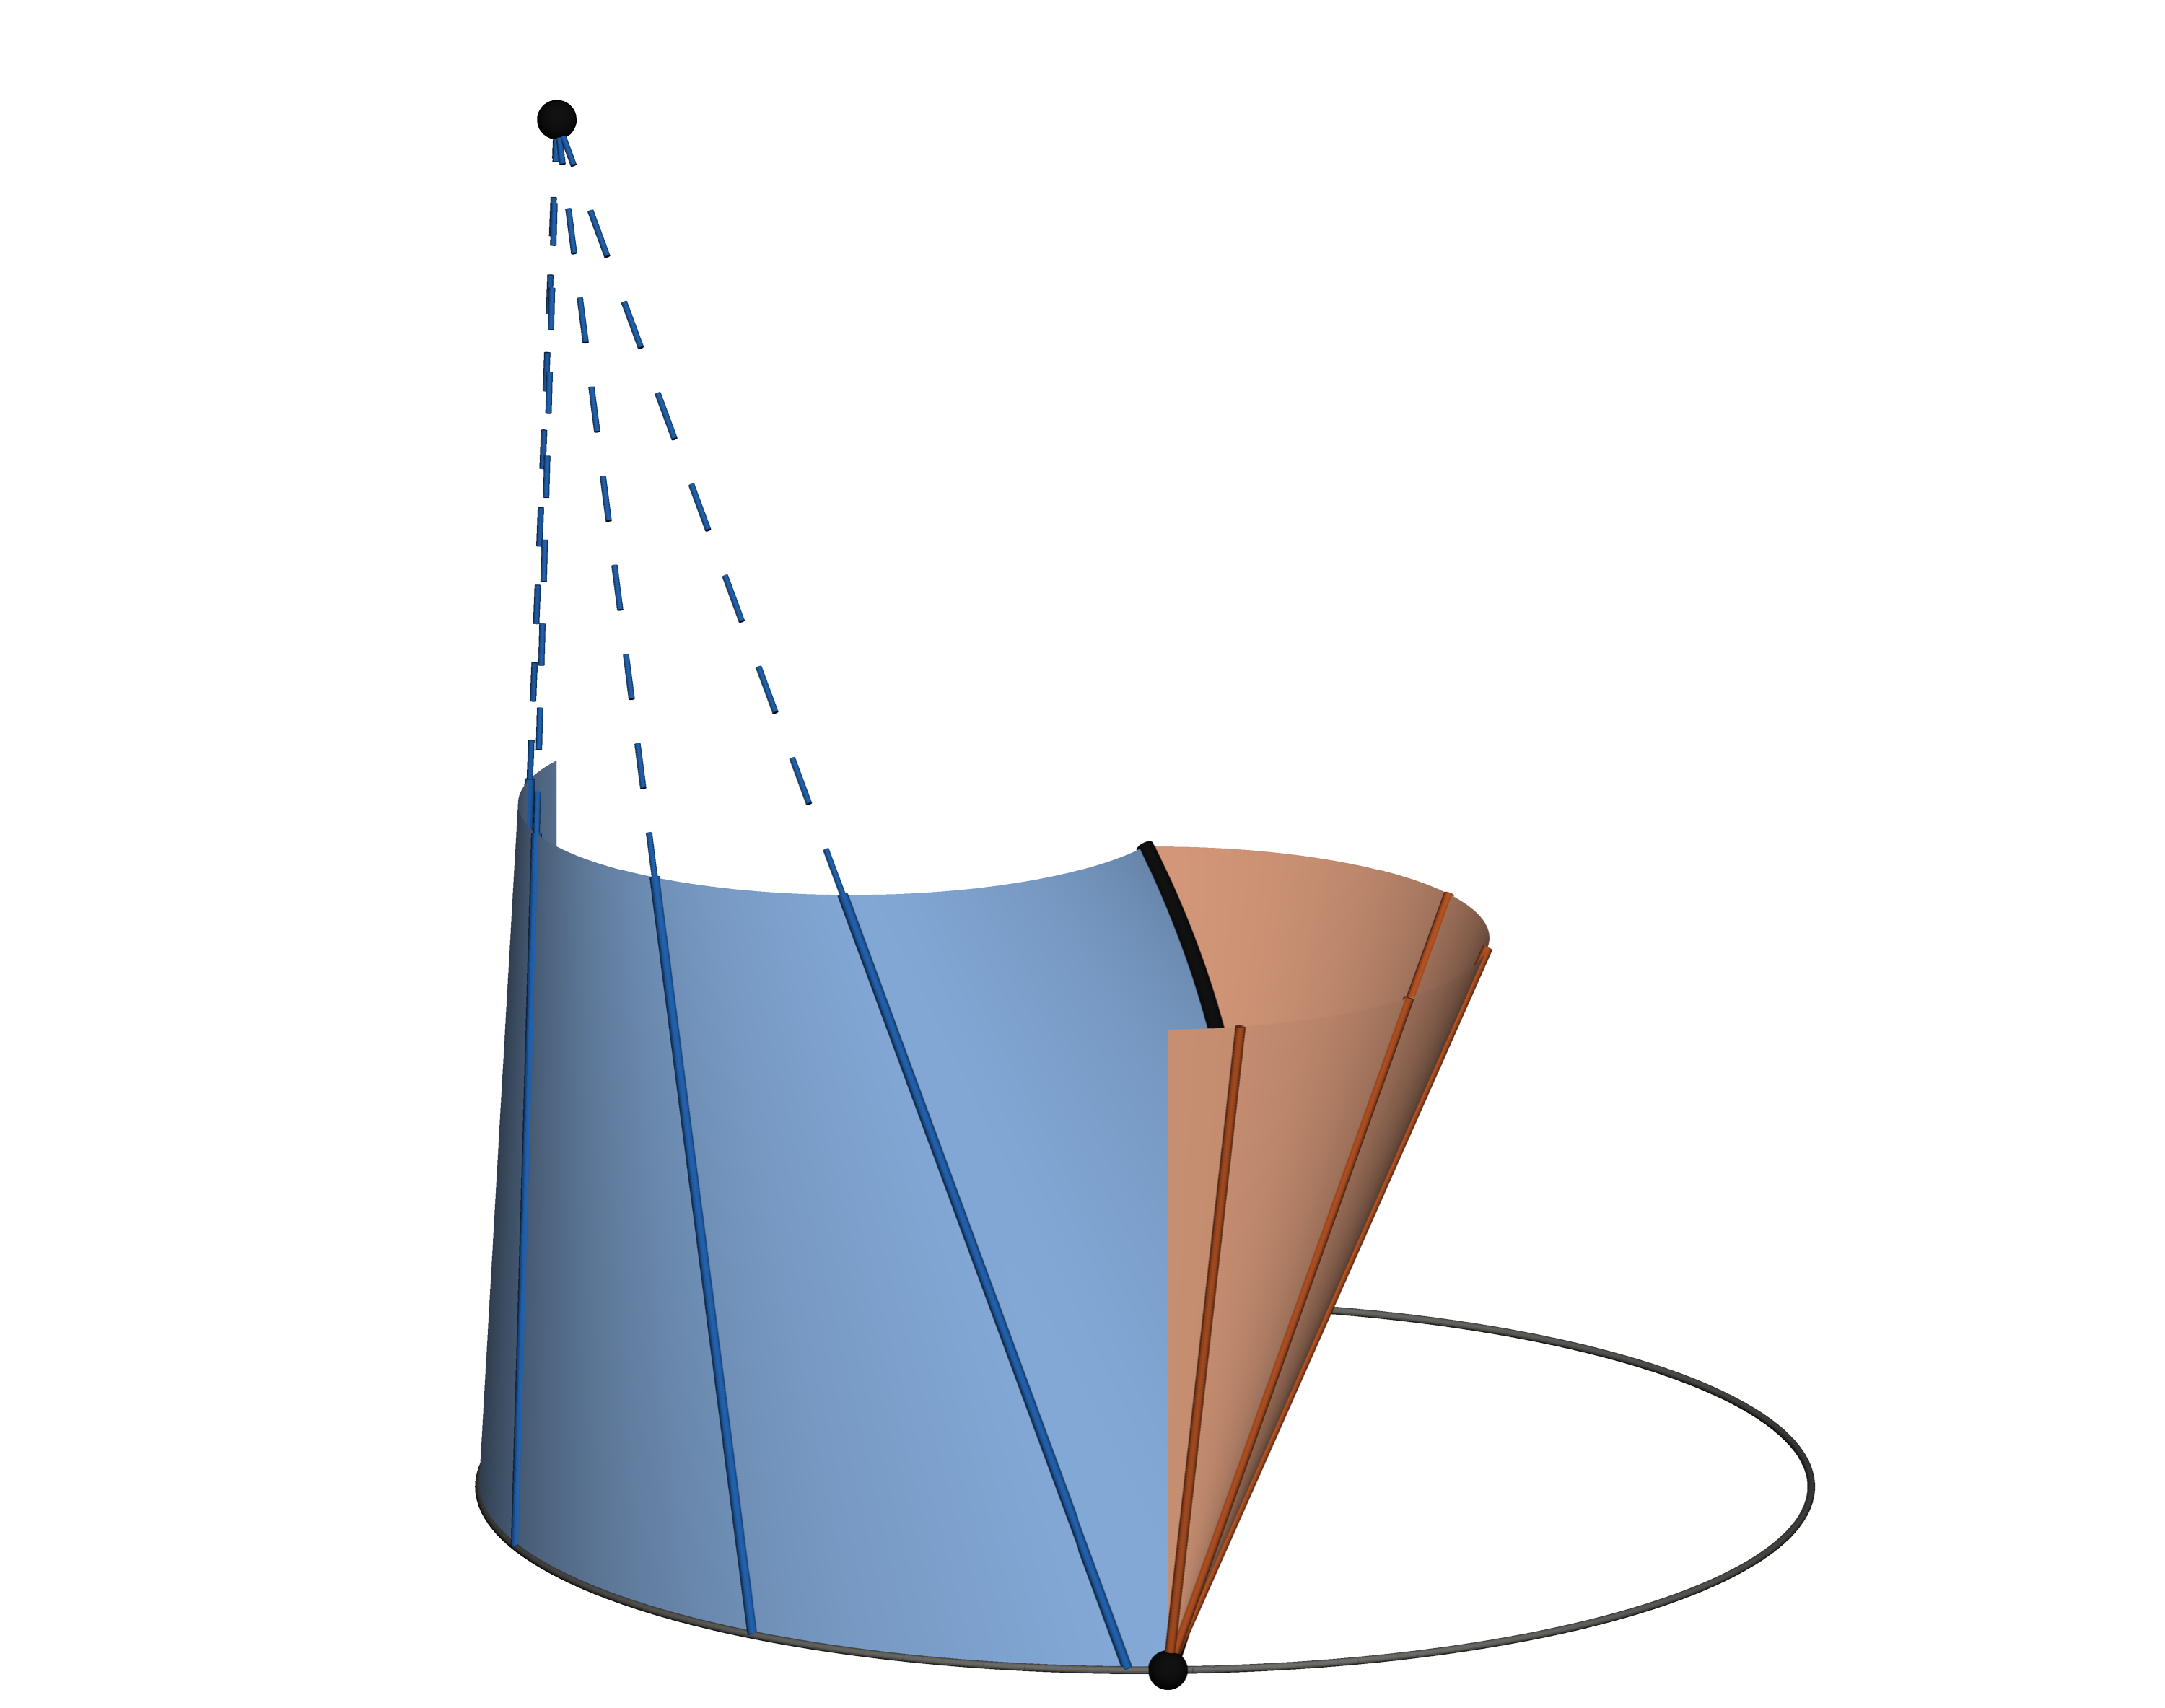
\includegraphics[width=0.43\textwidth]{figures/leaflet3d_a.png}};
\begin{scope}[x={(a.south east)}, y={(a.north west)}]
  \node[lab, anchor=west, xshift=3pt] at (\labAVone) {$V_1=(-1,0,2)$};
  \node[lab, anchor=north west, xshift=2pt] at (\labAVtwo) {$V_2=P$};
  \draw[inktwo, line width=0.4pt] (\labAM) -- ++(0.1,0.13) node[lab, anchor=south west, inner sep=1pt] {$M(z)$};
  \node[lab, anchor=east, xshift=-6pt] at (\labAE) {$E$};
  \node[panel, anchor=north west] at (0,1) {(a)};
\end{scope}
\node[anchor=south west, inner sep=0] (b) at ($(a.south east)+(0.1\textwidth,0)$)
  {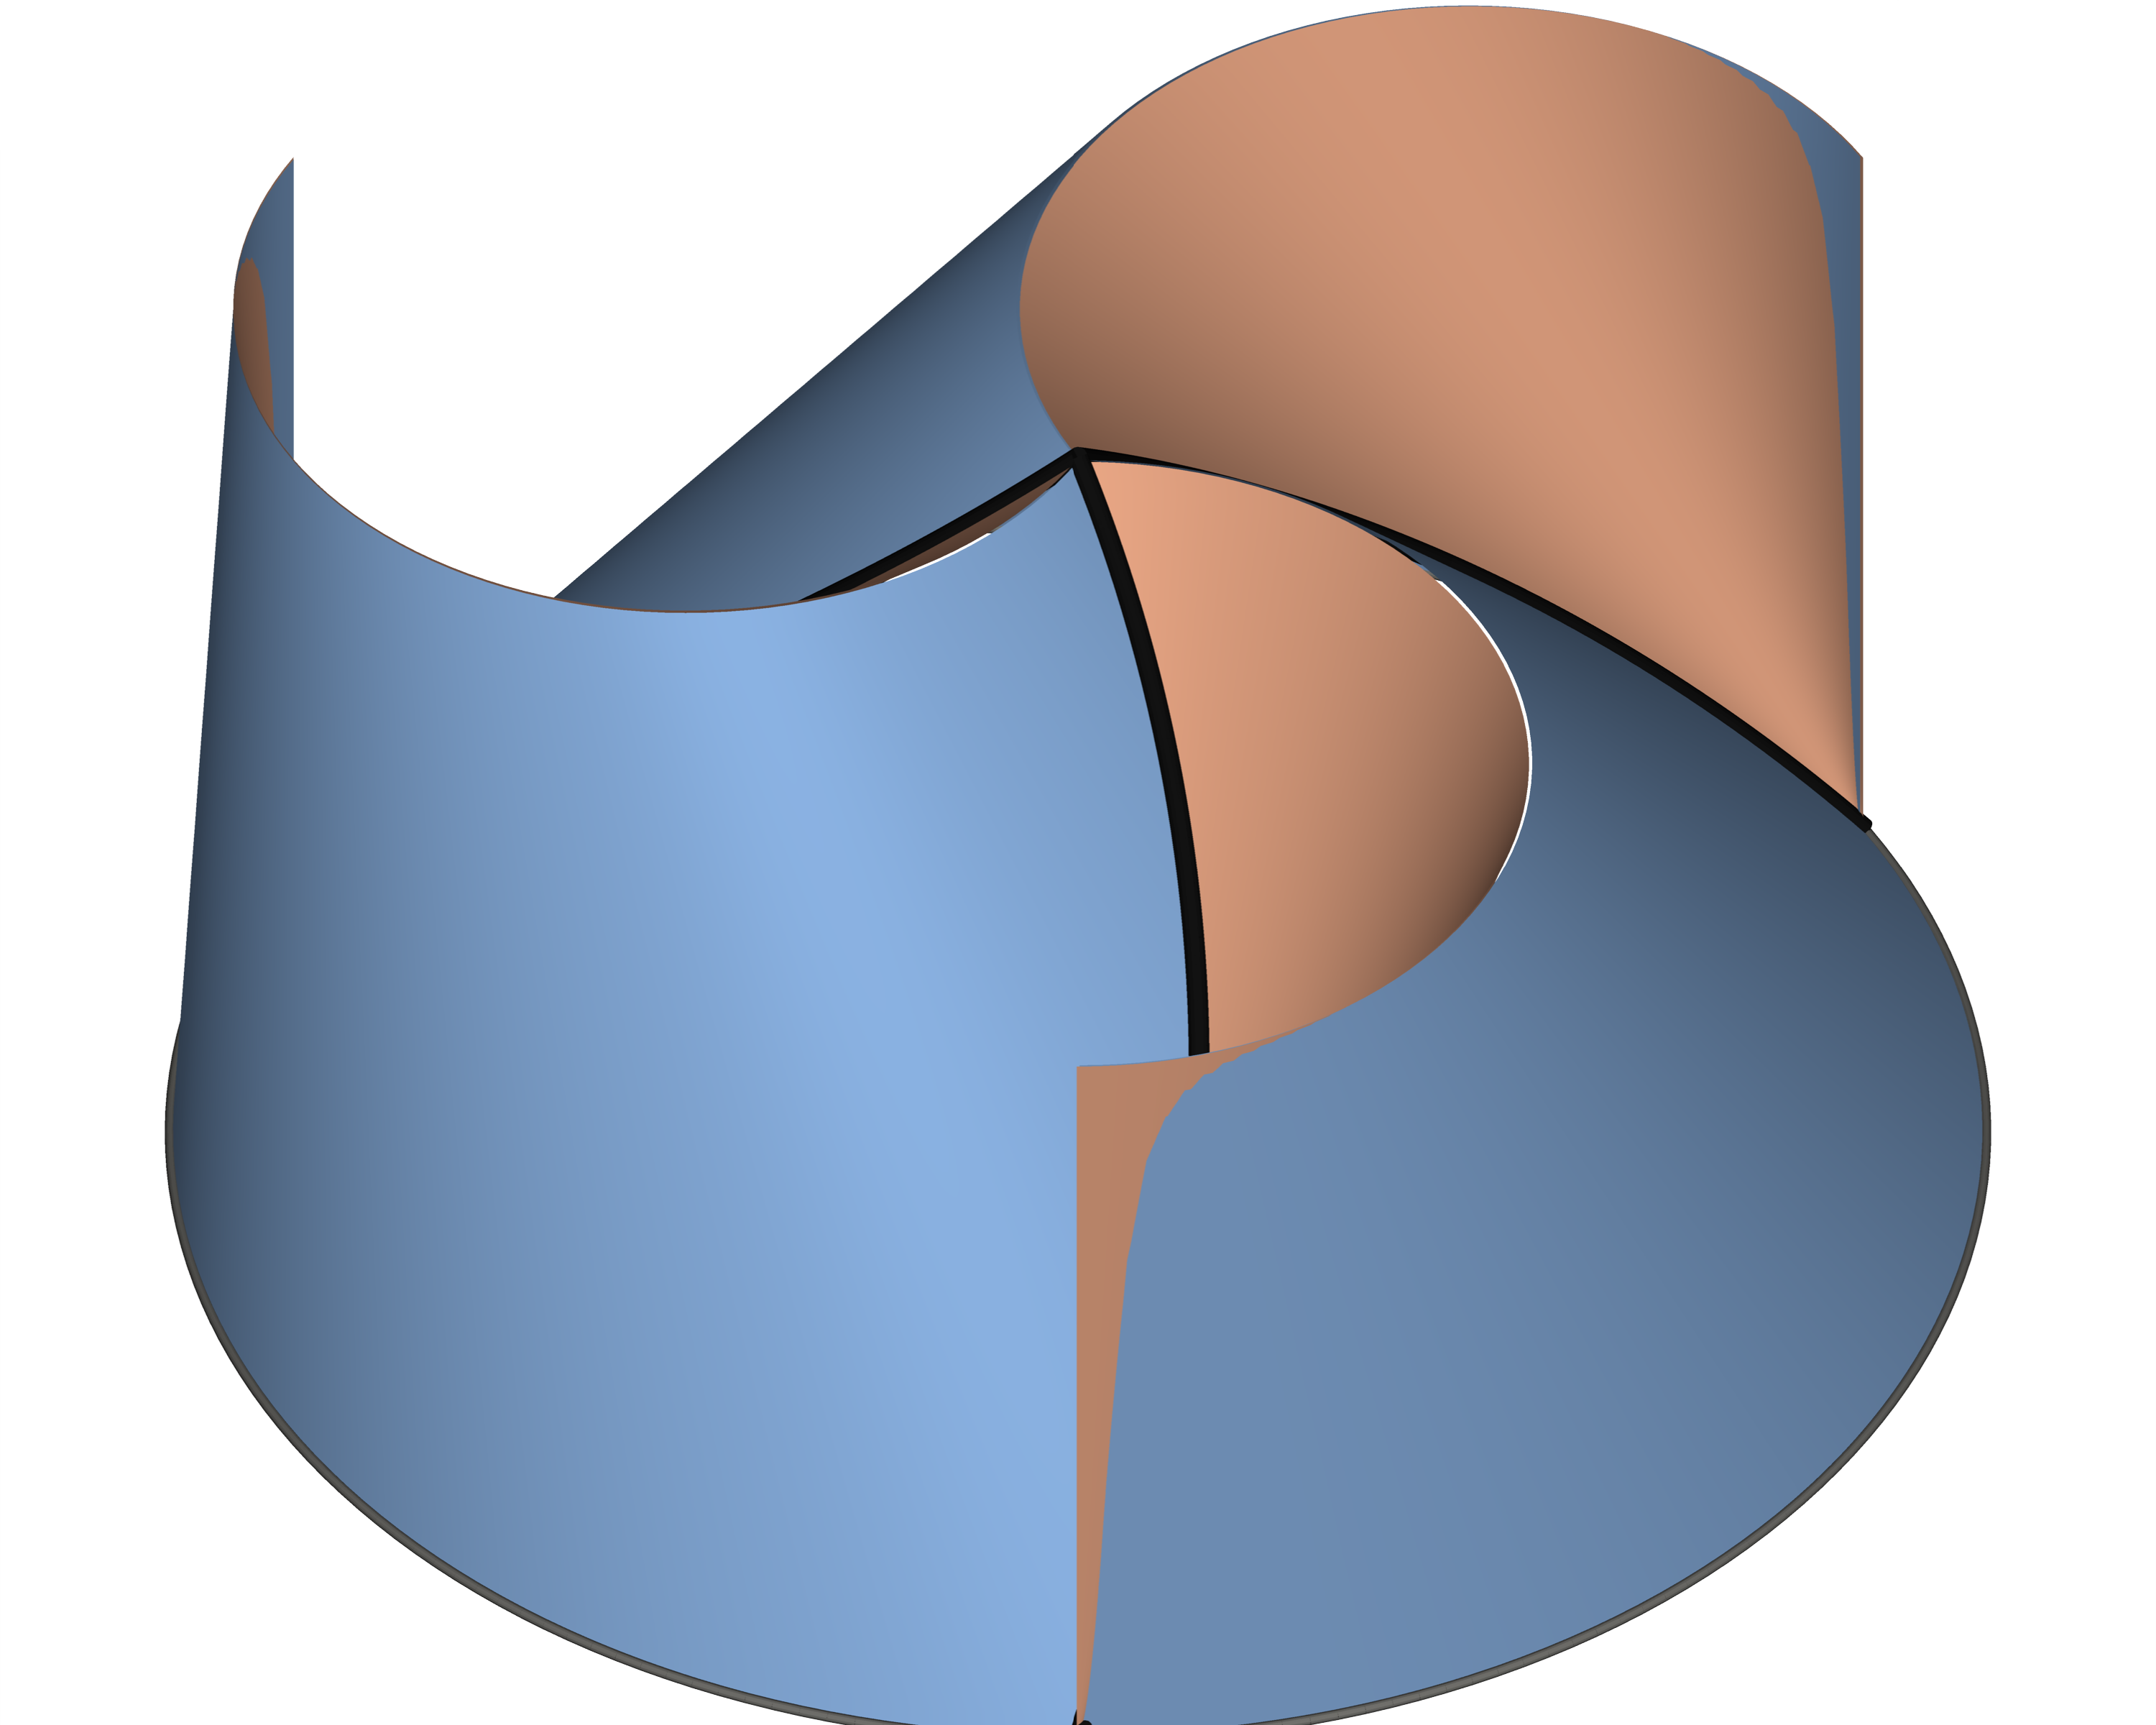
\includegraphics[width=0.43\textwidth]{figures/leaflet3d_b.png}};
\begin{scope}[shift={(b.south west)}, x={($(b.south east)-(b.south west)$)}, y={($(b.north west)-(b.south west)$)}]
  \node[lab, halo, anchor=south, yshift=3pt] at (\labBO) {$O$};
  \node[panel, anchor=north west] at (-0.08,1) {(b)};
\end{scope}
\end{tikzpicture}
